\documentclass{beamer}
%
% Choose how your presentation looks.
%
% For more themes, color themes and font themes, see:
% http://deic.uab.es/~iblanes/beamer_gallery/index_by_theme.html
%


\mode<presentation>
{
  \usetheme{Madrid}      % or try Darmstadt, Madrid, Warsaw, ...
  \usecolortheme{default} % or try albatross, beaver, crane, ...
  \usefonttheme{default}  % or try serif, structurebold, ...
  \setbeamertemplate{navigation symbols}{}
  \setbeamertemplate{caption}[numbered]

} 
\usepackage{amsmath,amssymb,amsthm,graphicx,float,subfigure,cite, pdflscape,color,setspace, xspace}
\usepackage{multimedia}
\usepackage[english]{babel}
\usepackage[utf8x]{inputenc}
\usepackage{hyperref}
%\hypersetup{
%	colorlinks   = true, %Colours links instead of boxes
%	urlcolor     = blue, %Colour for external hyperlinks
%	linkcolor    = blue, %Colour of internal links
%	citecolor   = red %Colour of citations
%}
\renewcommand{\familydefault}{\sfdefault}  % say no to serif
%\usepackage{media9}

\newcommand{\ca}{Ca$^{2+}$\xspace}

\title[GNU Parallel]{Using GNU parallel: An introduction}
\author[Emma McIvor]{Emma McIvor}
\institute{University of Nottingham}
\date{\today}

\begin{document}

\begin{frame}
  \titlepage
\end{frame}

% Uncomment these lines for an automatically generated outline.
%\begin{frame}{Outline}
% \tableofcontents
%\end{frame}

%%%%%%
\begin{frame}{Outline}
\begin{itemize}
\item What is GNU parallel?
\item Building a basic example
\item Future: build a basic example in Julia?
\end{itemize}
\end{frame}

\begin{frame}{What is GNU parallel and why use it?}
\begin{itemize}
	\item GNU parallel is a tool that can execute independent jobs (e.g. a script to run a simulation) in parallel using one or more computers
	\item To run GNU parallel we create a shell file (\texttt{.sh}) that wraps the script we want to execute. This is good because it means we are not adding extra complexity into the simulation script (more complexity $\implies$ more chance of introducing errors!)
	\item GNU parallel allows us to run multiple simulations simultaneously which can be useful for reducing the overall computation time required e.g. doing parameter scans
\end{itemize}
\end{frame}

\begin{frame}{Setting up GNU parallel}
\begin{itemize}
\item See README.md on GitHub \url{https://github.com/emmamcivor/UoN_math_computing_seminar}
\item See GNU parallel documentation for additional installation help
\item All files used today are available from the GitHub repo so you can practise and make your own scripts to be run in parallel
\end{itemize}
\end{frame}

\begin{frame}{Running GNU parallel}
\begin{enumerate}
\item Make a working directory with the script you want to run in parallel e.g. \texttt{test.m}
\item Make a parameter list in a \texttt{parameter.txt} file with one set of parameters per line inside the working directory
\item Create the shell scripts to run GNU parallel
\begin{itemize}
\item These don't have to be placed in the working directory
\item I have placed them in the level above the working directory but I have added this folder to the local path on my \texttt{.bashrc} so I can run these shell scripts from the command line
\end{itemize}
\item \texttt{cd} into working directory and run shell script to run GNU parallel from command line
\end{enumerate}
\end{frame}

\begin{frame}{Example: Create a basic Matlab script}
This Matlab script (\texttt{test.m}) takes input parameters $a$ and $b$ and does a simple addition and multiplication which is saved to a unique file. We want to run this simulation for multiple pairs of parameter values.
\begin{figure}
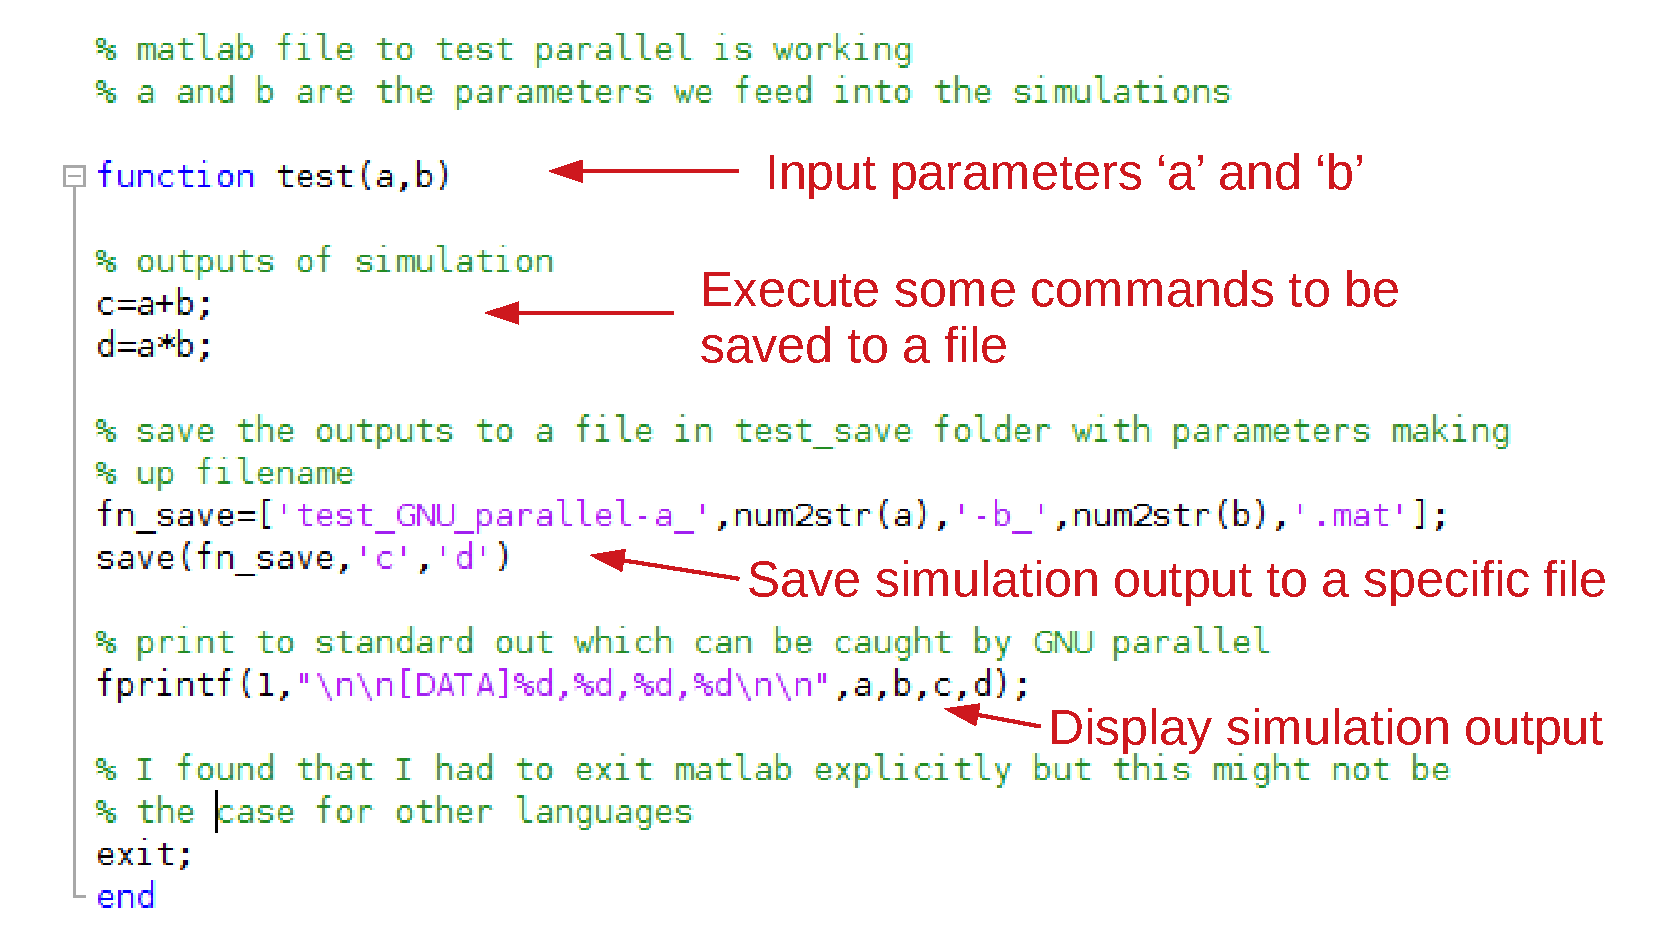
\includegraphics[width=.8\linewidth]{figures/matlab_code_annotated.pdf}	
\end{figure}
\end{frame}

\begin{frame}{Example: Create a parameter file with all necessary parameters}
\begin{itemize}
\item Create a file called \texttt{parameters.txt} containing all the parameters for the simulation
\item Each line is a set of parameters
\item I am using a comma separated format (I tell GNU parallel this later)
\end{itemize}
\begin{figure}
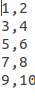
\includegraphics[width=.05\linewidth]{figures/parameter_file.png}
\end{figure}
\end{frame}

\begin{frame}{Example: Create a shell script to run a single instance of the Matlab script}
\begin{itemize}
	\item Create a new shell script (\texttt{run\_test\_matlab.sh}) to initiate the Matlab simulation:
\begin{figure}
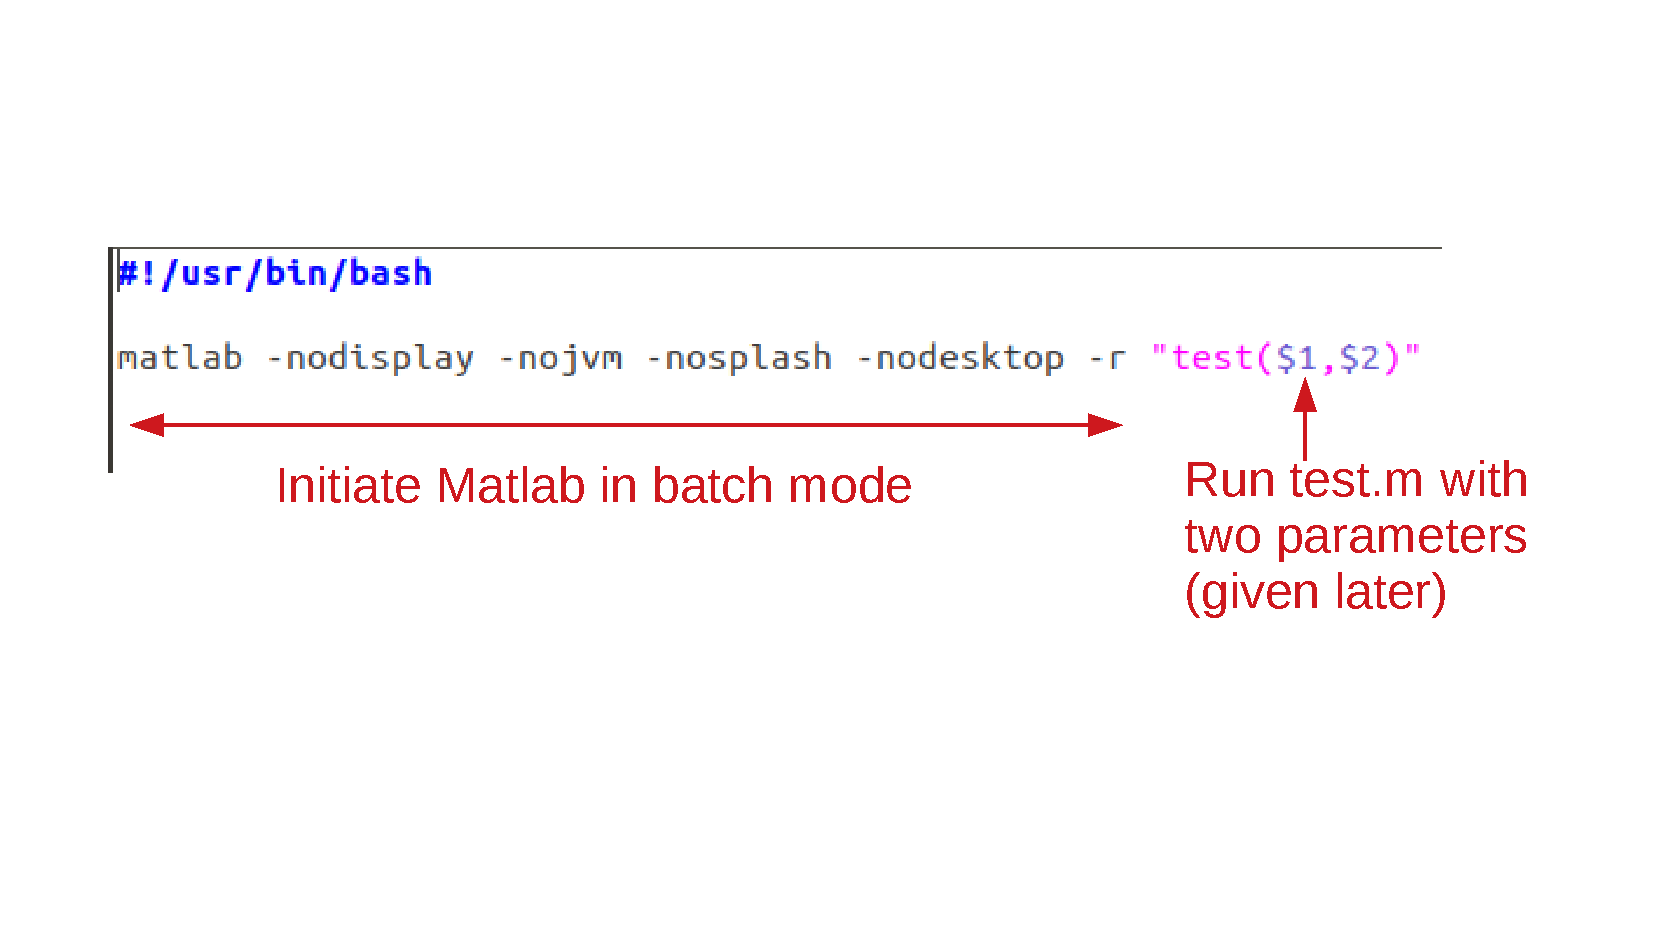
\includegraphics[clip,trim=0in 2in 0in 2in,width=0.8\linewidth]{figures/run_matlab_sh_annotated.pdf}
\end{figure}
\item Make sure this file is executable. If not, on the command line execute \\ \texttt{chmod u=rwx run\_test\_matlab.sh}
\end{itemize}
\end{frame}

\begin{frame}{Example: Create a shell script to run multiple simulations in parallel}
\begin{itemize}
\item Create a new shell script (\texttt{test\_parallel\_1host.sh}) to run the Matlab simulations simultaneously/in parallel:
\begin{figure}
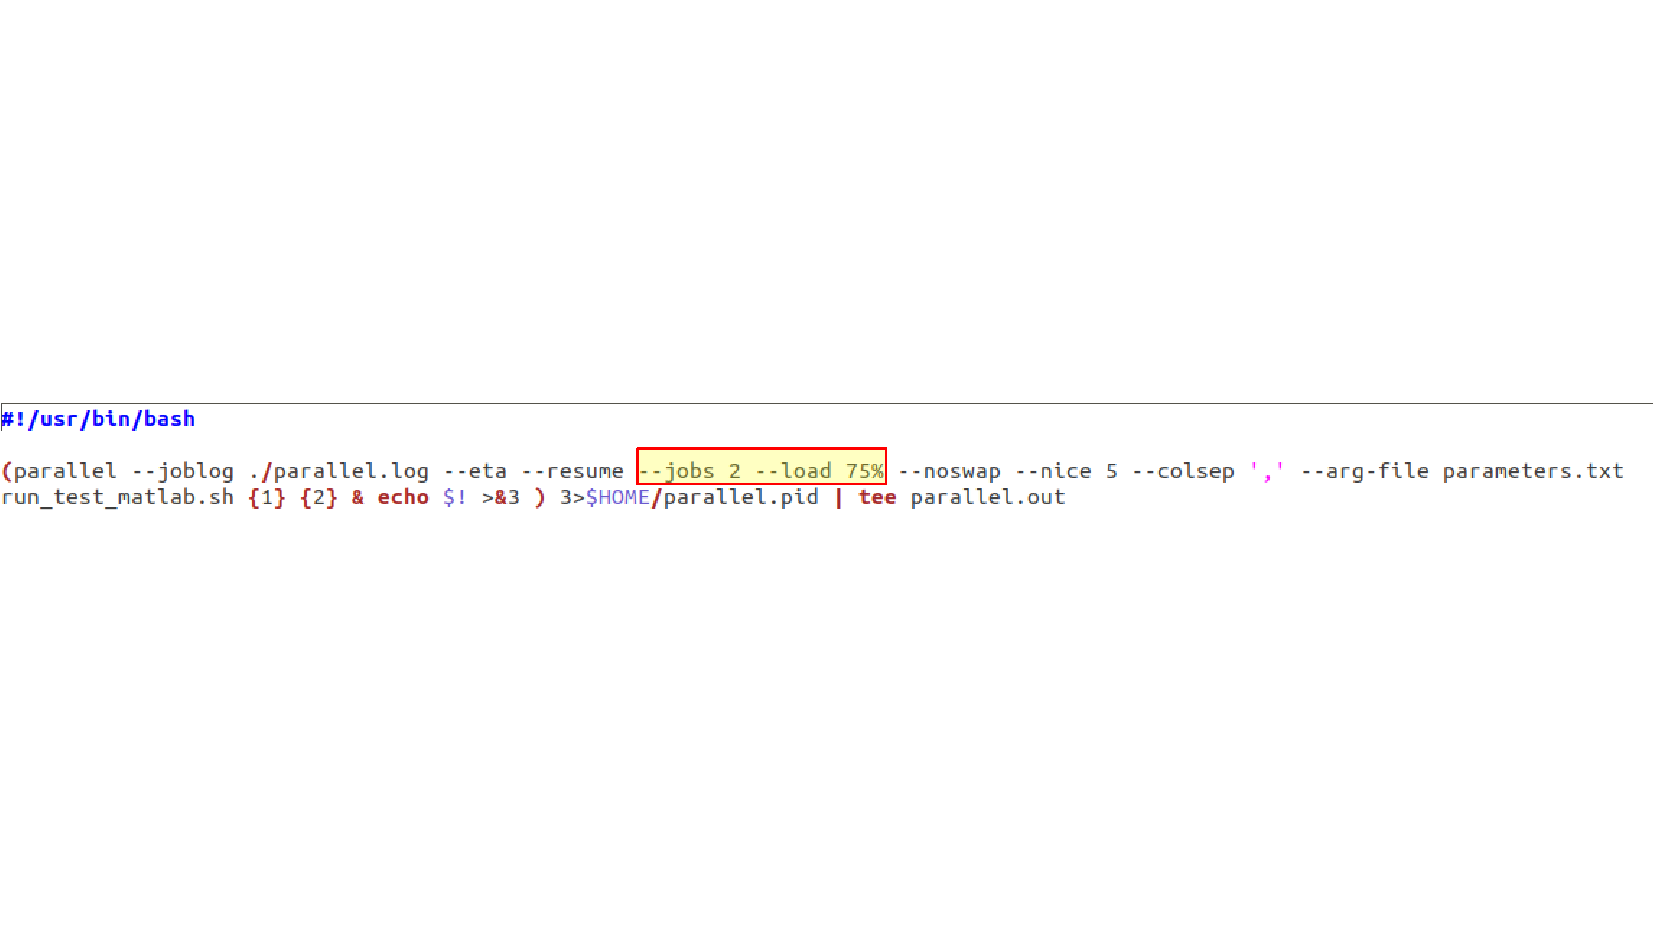
\includegraphics[clip,trim=0in 2.5in 0in 2.5in,width=\linewidth]{figures/run_parallel_annotated.pdf}
\end{figure}
\item Make sure this file is executable. If not, on the command line execute \\ \texttt{chmod u=rwx test\_parallel\_1host.sh}
\item This command is explained in deatil in the README.md of this repository and in GNU parallel documentation
\end{itemize}
\end{frame}

\begin{frame}[fragile]{Example: Make sure both shell scripts can be found on local path}
This allows us to run the shell script inside any folder containing the Matlab script and parameter list. To do this:
\begin{itemize}
\item Suppose shell scripts are in the folder \texttt{{\raise.17ex\hbox{$\scriptstyle\mathtt{\sim}$}}/work/math\_server\_talks}
\item Open the \texttt{.bashrc} file e.g. \texttt{gedit {\raise.17ex\hbox{$\scriptstyle\mathtt{\sim}$}}/.bashrc}
\item Modify the PATH to include this folder e.g. 
\small
\begin{verbatim}
export PATH=$HOME/local/bin:$HOME/work/math_server_talks:$PATH
\end{verbatim}
\item Reload your .bashrc file so that the PATH is updated \\
\texttt{. ./.bashrc}
\end{itemize}
\end{frame}

\begin{frame}[fragile]{Example: Run GNU parallel}
\begin{itemize}
	\item Make sure \texttt{test.m} and \texttt{parameters.txt} are in the current working directory (\texttt{{\raise.17ex\hbox{$\scriptstyle\mathtt{\sim}$}}/work/math\_server\_talks/example1})
	\item Execute \texttt{test\_parallel\_1host.sh} on the command line to run $5$ Matlab simulations, $2$ at a time.
	\item As one simulation finishes GNU parallel automatically spawns the next simulation in the queue
	\item Execute \texttt{clean\_stdout.sh} to extract the data displayed in standard out and save it in a comma separated list (if you want)
\item \textbf{If you use GNU parallel you should cite the software}:
\tiny
\begin{verbatim}
@book{tange_ole_2018_1146014,
      author       = {Tange, Ole},
      title        = {GNU Parallel 2018},
      publisher    = {Ole Tange},
      month        = Mar,
      year         = 2018,
      ISBN         = {9781387509881},
      doi          = {10.5281/zenodo.1146014},
      url          = {https://doi.org/10.5281/zenodo.1146014}
}
\end{verbatim}
\end{itemize}
\end{frame}

%\begin{frame}{Background on concurrency and parallelism}
%\url{https://vimeo.com/49718712}
%\end{frame}


\end{document}

%\begin{figure}
%	\subfigure[]{\includegraphics[clip,trim=2.5in 0in 2.5in 0in, width=0.3\linewidth]{bio_model_orai_influx_no_PMCA.pdf}
%		\label{fig:intro:ill:Orai_influx}			
%	}	
%	\subfigure[]{\includegraphics[clip,trim=2.5in 0in 2.5in 0in, width=0.3\linewidth]{bio_model_activated_pumps_no_PMCA.pdf}
%		\label{fig:intro:ill:Orai_influx_SERCA_uptake}
%	}		
%	\subfigure[]{\includegraphics[clip,trim=2.5in 0in 2.5in 0in, width=0.3\linewidth]{bio_model_refill_no_PMCA.pdf}
%		\label{fig:intro:ill:Refilling}
%	}	
%	\caption{(a) Orai channels on PM open. (b) Increased \ca in ER-PM junction activates SERCA pumps on ER membrane. (c) Activated SERCA pumps refill ER}		
%\end{figure}
